%%%%%%%%%%%%%%%%%%%%%%%%%%%%%%%%%%%%%%%%%
% a0poster Portrait Poster
% LaTeX Template
% Version 1.0 (22/06/13)
%
% The a0poster class was created by:
% Gerlinde Kettl and Matthias Weiser (tex@kettl.de)
% 
% This template has been downloaded from:
% http://www.LaTeXTemplates.com
%
% License:
% CC BY-NC-SA 3.0 (http://creativecommons.org/licenses/by-nc-sa/3.0/)
%
%%%%%%%%%%%%%%%%%%%%%%%%%%%%%%%%%%%%%%%%%

%----------------------------------------------------------------------------------------
%	PACKAGES AND OTHER DOCUMENT CONFIGURATIONS
%----------------------------------------------------------------------------------------

\documentclass[a0,portrait]{a0poster}
\usepackage{multicol}
\usepackage[svgnames]{xcolor}
% \usepackage{times}
\usepackage{graphicx}
\graphicspath{{figures/}}
\usepackage{booktabs}
\usepackage[font=small,labelfont=bf]{caption}
\usepackage{amsfonts, amsmath, amsthm, amssymb}
\usepackage{wrapfig}
\usepackage{indentfirst}
\usepackage{enumitem}
\usepackage{tikz}
\usetikzlibrary{shapes.geometric, arrows, positioning, fit, backgrounds}
\usepackage{hyperref}
\usepackage{framed}
\usepackage{wrapfig}



% \usepackage[showframe]{geometry} % having difficulty getting this to work

% \usepackage{fancyhdr} % also having trouble with fancyhdr
% See Overleaf documentation 'Headers and footers: using the fancyhdr package'
% \pagestyle{fancy}
% \fancyhf{} % clear existing header/footer entries
% \fancyfoot[L]{adsf}
% \fancyfoot[R]{%\begin{center}
% \begin{tabular}{cc}
% \raisebox{-0.2\height}{
\includegraphics[height=1cm]{cc-by.png}} &
% \raisebox{0.2ex}{\small This work is licensed under a Creative Commons Attribution 4.0 International License.}
% \end{tabular}
% %\end{center}
% }

\usepackage{fontspec}
\usepackage[english, bulgarian]{babel}
\usepackage{polyglossia}

\usepackage{microtype}
\newfontfamily{\cyrillicfont}{NewCM10-Regular} 
\setdefaultlanguage{english}
\setotherlanguages{russian}
%https://tex.stackexchange.com/a/669979

% \usepackage[style=authoryear,backend=biber,heading=bibintoc]{biblatex}
% \addbibresource{references.bib}
\usepackage{caption}
\newenvironment{Figure}
  {\par\medskip\noindent\minipage{\linewidth}}
  {\endminipage\par\medskip}
%https://tex.stackexchange.com/a/12289

% Define ARDC colors
\definecolor{ARDCBlue}{RGB}{0,159,218}
\definecolor{ARDCPink}{RGB}{236,0,140}
\definecolor{ARDCYellow}{RGB}{255,194,14}
\definecolor{ARDCPurple}{RGB}{146,39,143}
\definecolor{DarkGrey}{RGB}{64,64,64}

% Set margins
% Use the geometry package for this, Shawn, this is why your footer doesn't work, I think.
\setlength{\topmargin}{2cm}
\setlength{\oddsidemargin}{2cm}
\setlength{\evensidemargin}{2cm}
\setlength{\textwidth}{0.95\paperwidth}
\setlength{\textheight}{0.975\paperheight}
\setlist[enumerate]{leftmargin=2em}

% Increase first-line indent
\setlength{\parindent}{2em}

\setmainfont{Arial}
% https://tex.stackexchange.com/questions/639067/defining-a-fallback-font-for-all-missing-characters

\begin{document}

%----------------------------------------------------------------------------------------
% POSTER HEADER
%----------------------------------------------------------------------------------------
\setlength{\columnsep}{2cm}

\begin{multicols}{2}

\noindent
\vspace{0pt}
\Huge \color{ARDCBlue} \textbf{The Research Activity Identifier (RAiD)} \color{Black}\\[0.3cm]
\Large\textit{System architecture, metadata schema, workflows, and examples}\\[1cm]
\large \textbf{Shawn Ross\textsuperscript{1}, Natasha Simons\textsuperscript{1}, Rob Leney\textsuperscript{1}, Steffen Weidenhaus\textsuperscript{1}}\\[0.5cm]
\large \textsuperscript{1}Australian Research Data Commons

\vfill\null
\columnbreak
\raggedleft
\noindent
\includegraphics[width=0.5\linewidth]{ARDC logo - RGB.png}

\end{multicols}     

\begin{multicols}{3}

%----------------------------------------------------------------------------------------
% BACKGROUND
%----------------------------------------------------------------------------------------
\color{ARDCPink}
\section*{\LARGE Background}
\color{DarkGrey}
\large{
\input background
}

%----------------------------------------------------------------------------------------
% Technical implementation
%----------------------------------------------------------------------------------------
\color{ARDCYellow}
\section*{\LARGE RAiD technical implementation}
\color{DarkGrey}
\large{
Each RAiD Registration Agency runs an instance of the RAiD Service, federated into the global RAiD System. It is designed to be scalable and re-deployable. 
}

% ---------------------------
% RAiD Architecture diagrams
% ---------------------------
% Add vertical space before the diagram

\vspace{1cm}

\centerline{\textbf{RAiD architecture}}
\begin{Figure}
  \centering
  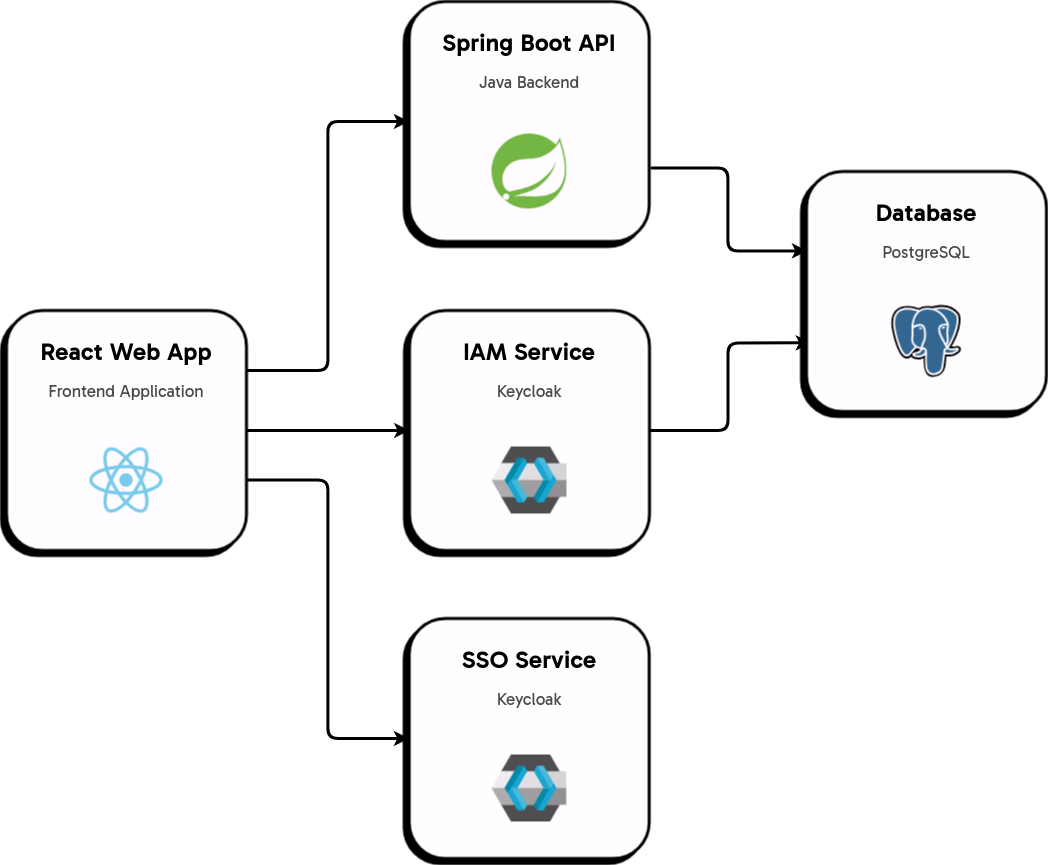
\includegraphics[width=0.75\linewidth]{figures/20241023-raid-architecture-appflow-basic.png}
  \captionof{figure}{RAiD is built using React, Spring Boot, Keycloak, and PostgreSQL.}
  \label{basic-architecture}
\end{Figure}

\vspace{1cm}

\centerline{\textbf{RAiD AWS implementation}}
\begin{Figure}
  \centering
  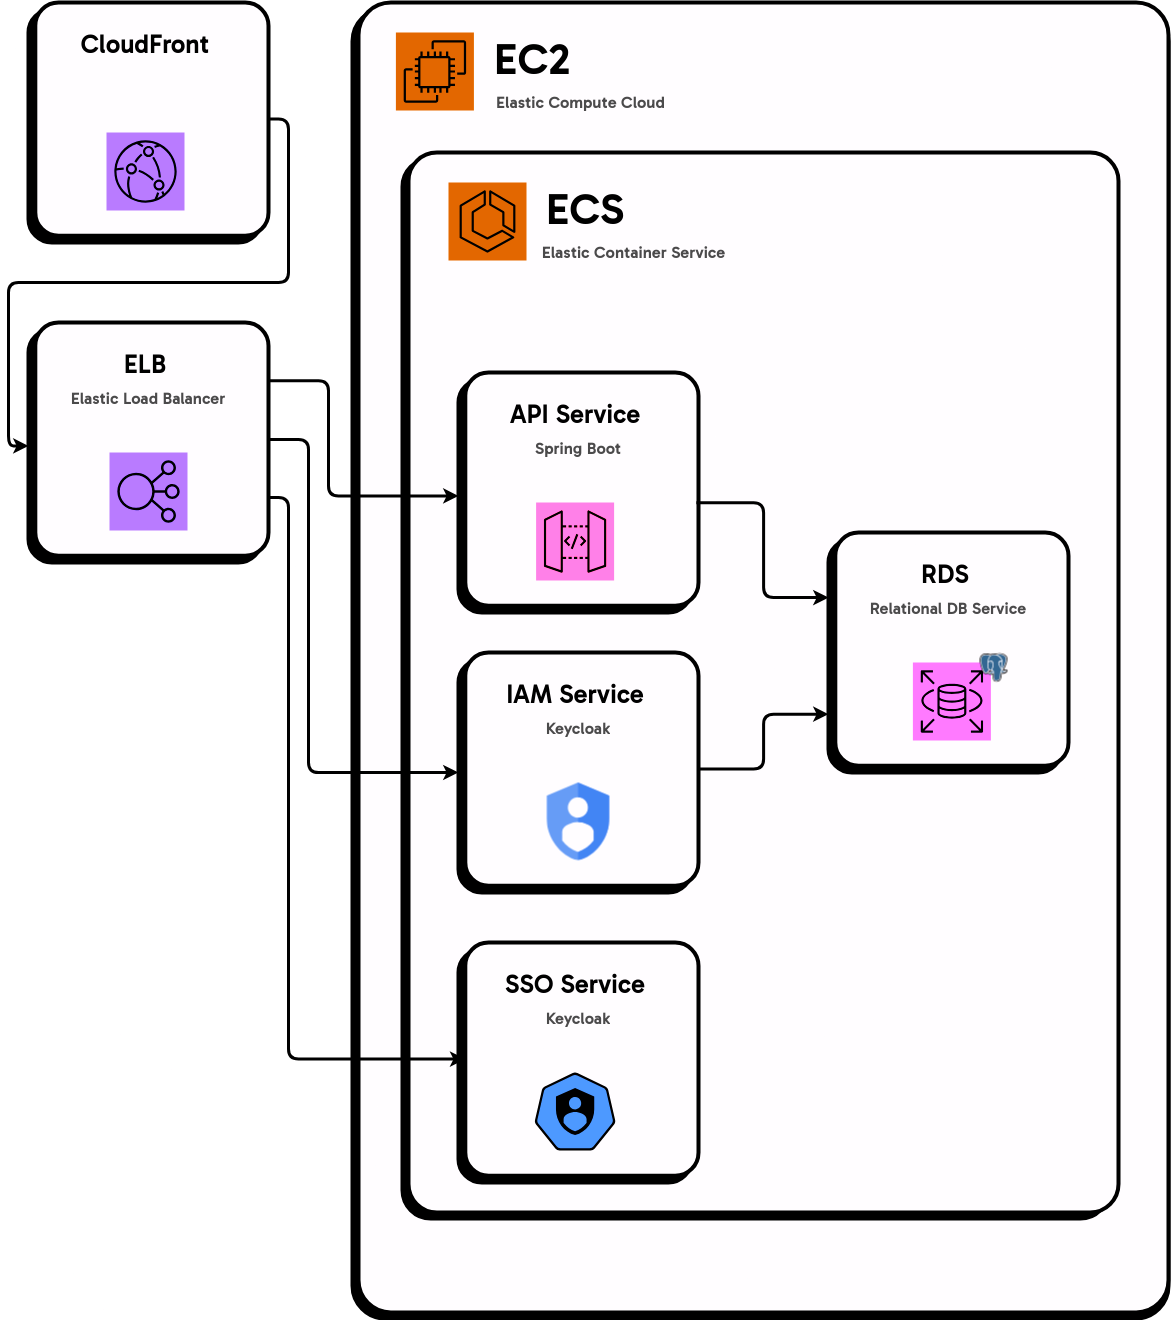
\includegraphics[width=0.75\linewidth]{figures/20241023-raid-architecture-appflow-aws.png}
  \captionof{figure}{RAiD leverages various AWS services.}
  \label{aws-architecture}
\end{Figure}

\vspace{1cm}

\centerline{\textbf{RAiD feature implementation}}
\begin{Figure}
  \centering
  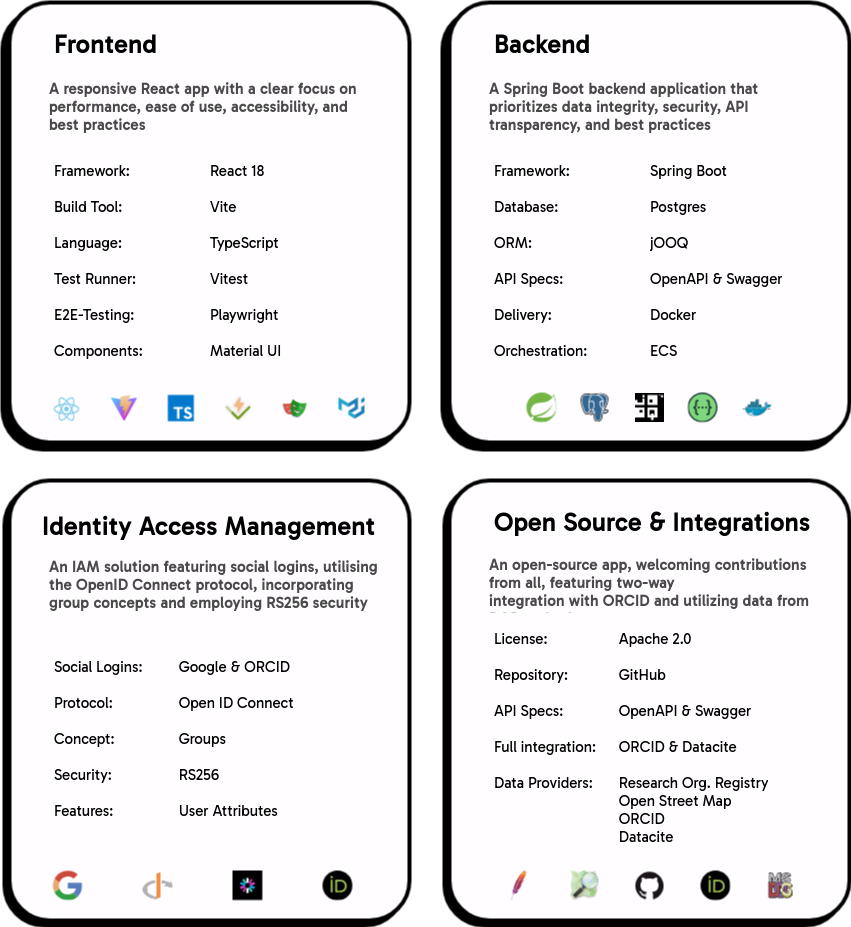
\includegraphics[width=0.75\linewidth]{figures/20241023-raid-architecture-feature-boxes.png}
  \captionof{figure}{RAiD architecture details.}
  \label{reature-implementation}
\end{Figure}


%----------------------------------------------------------------------------------------
% Key RAiD features
%----------------------------------------------------------------------------------------

\color{ARDCPurple}
\section*{\LARGE A project-focused system}
\color{DarkGrey}
\large{
RAiD has been designed from the ground up as a dedicated research project identifier. In addition to serving as a PID for projects, it is also a registry and a collaborative metadata management system.
}

\vspace{0.5cm}

\begin{Figure}
  \centering
  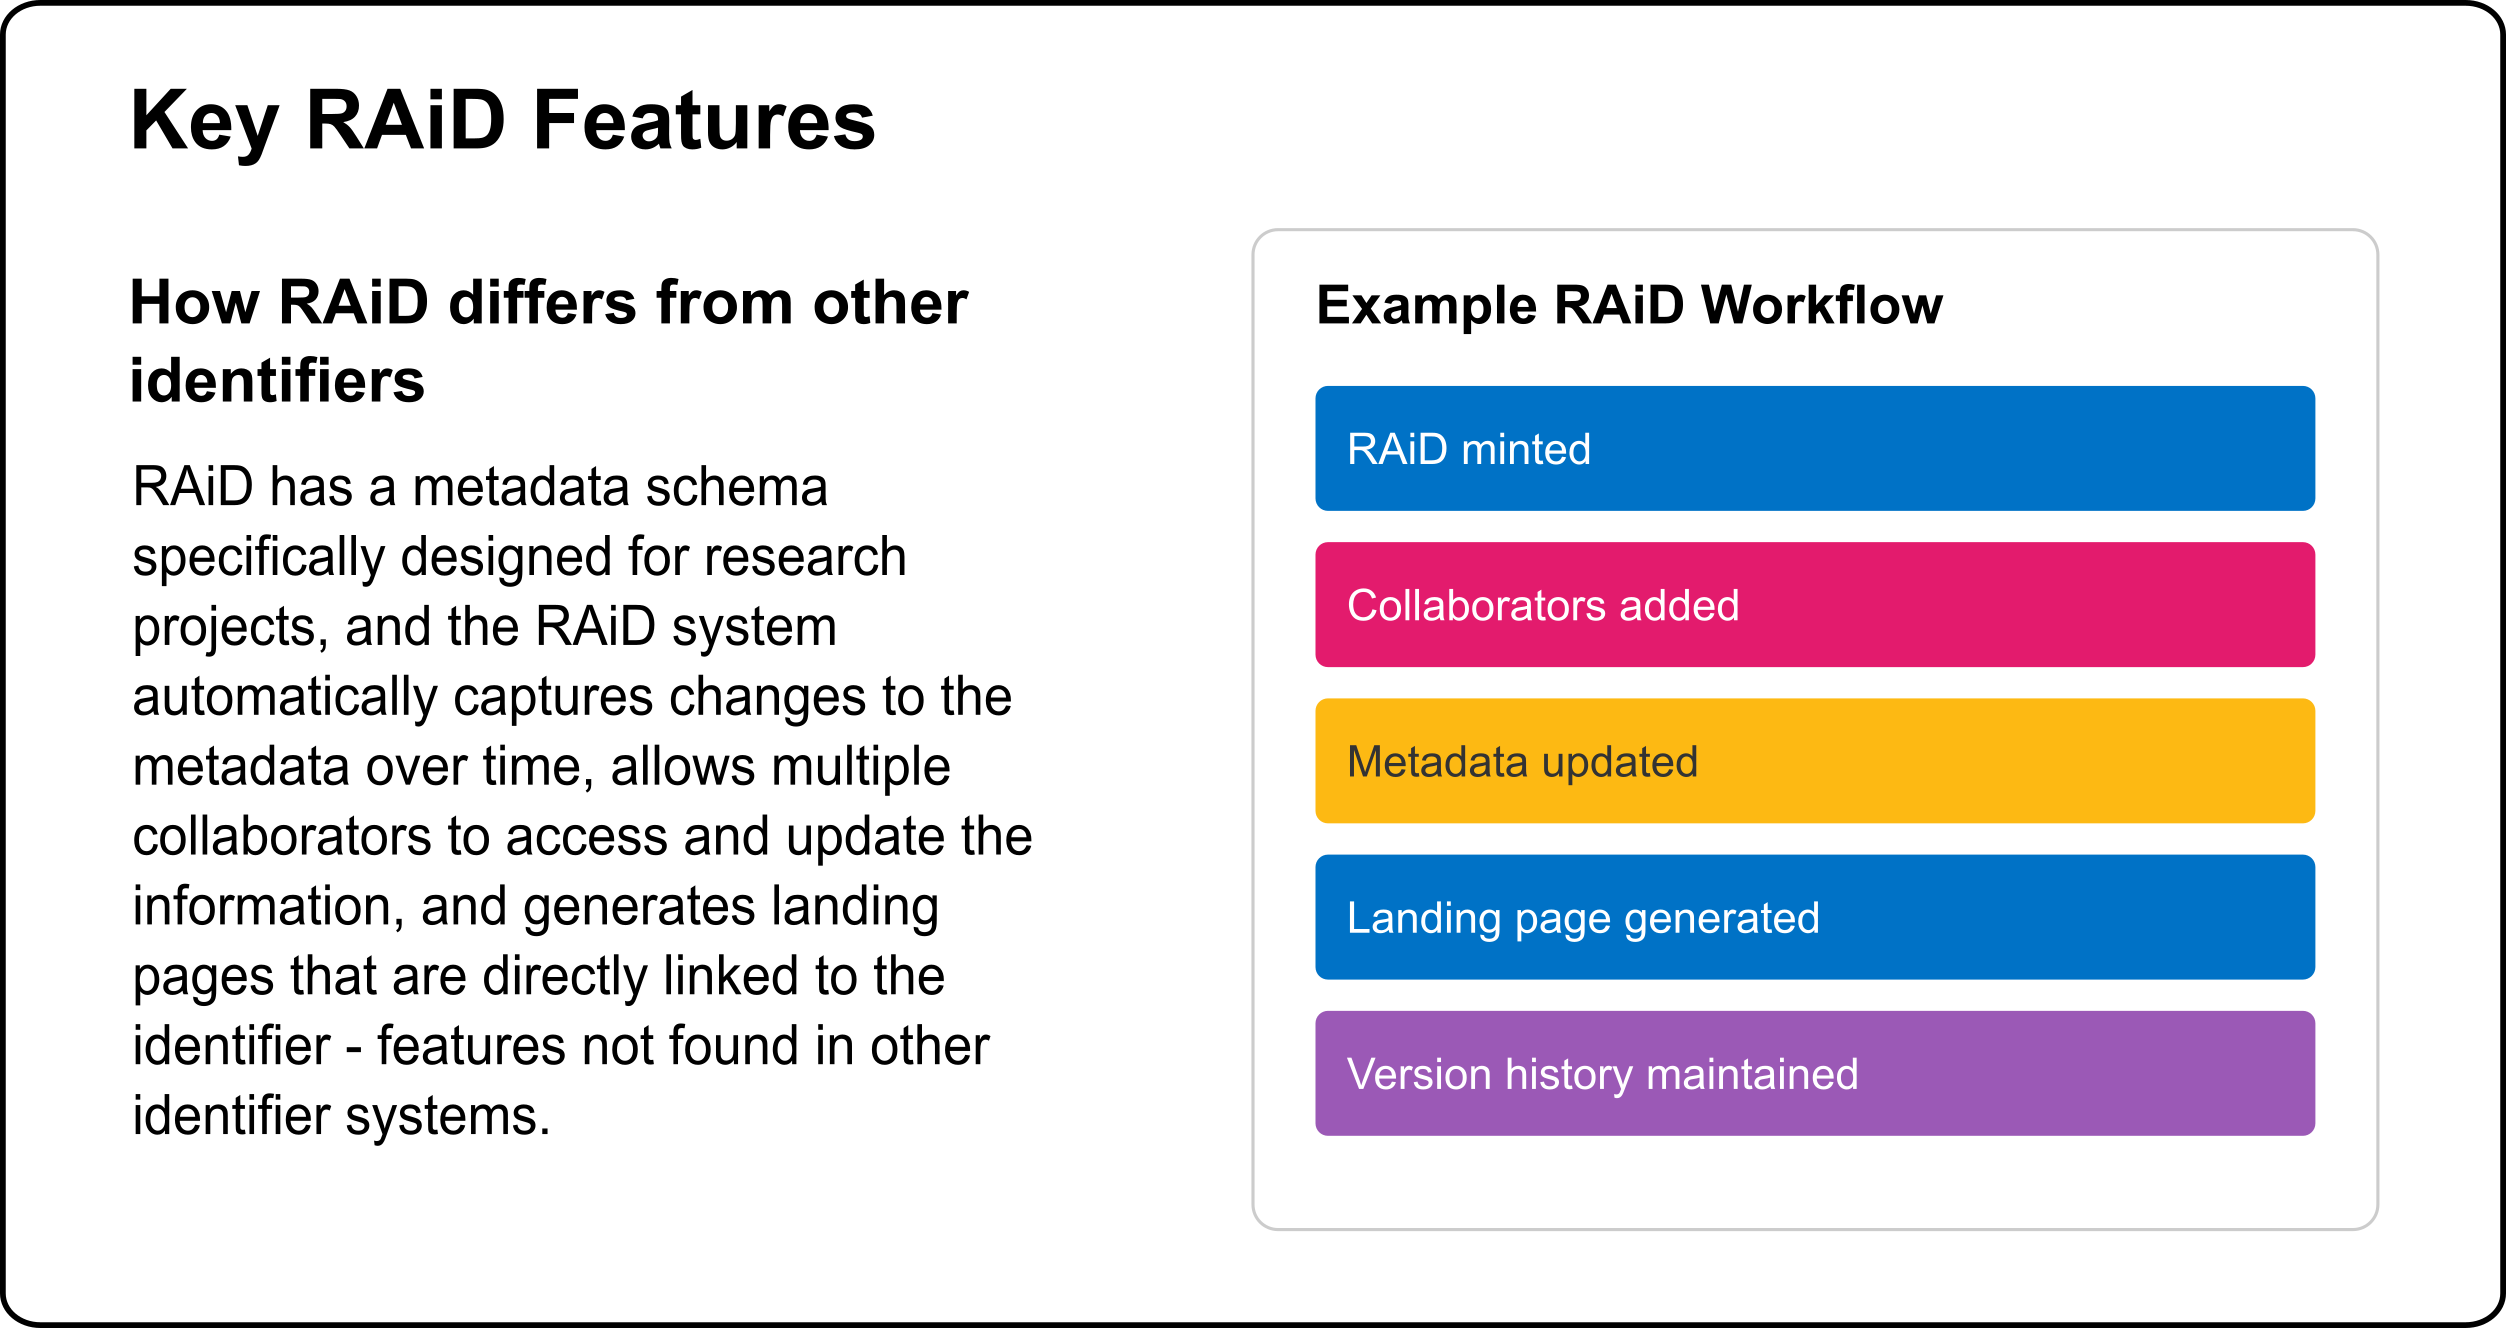
\includegraphics[width=0.9\linewidth]{figures/raid-key-features.png}
  \label{key-features}
\end{Figure}

%----------------------------------------------------------------------------------------
% Acquiring RAiD - Europe
%----------------------------------------------------------------------------------------

% \vspace{-1cm}
% 
% \color{ARDCBlue}
% \section*{\LARGE How to get RAiD (Europe)}
% \color{DarkGrey}
% \large{
% SURF is the RAiD Registration Agency for Europe. Researchers acquire RAiDs through their organisations or through integrations with services like the EOSC Marketplace. 

% In most cases, the first step to using RAiD is for your organisation to establish a relationship with SURF. Email \href{mailto:raid@surf.nl}{raid@surf.nl} to get started.

%----------------------------------------------------------------------------------------
% Acquiring RAiD - ANZ
%----------------------------------------------------------------------------------------

\vspace{-1cm}

\color{ARDCBlue}
\section*{\LARGE How to get RAiD (ANZ)}
\color{DarkGrey}
\large{
The ARDC is the RAiD Registration Agency for Australia and New Zealand. Researchers acquire RAiDs through their organisations. The first step to using RAiD is for your organisation to establish a relationship with the ARDC. Members of the ARDC DataCite Consortium may utilise RAiD immediately. Email \href{mailto:contact@raid.org}{contact@raid.org} to get started. 
}

%----------------------------------------------------------------------------------------
% 'Getting started with RAiD in Australia and New Zealand' figure
%----------------------------------------------------------------------------------------
\begin{Figure}
 \centering
 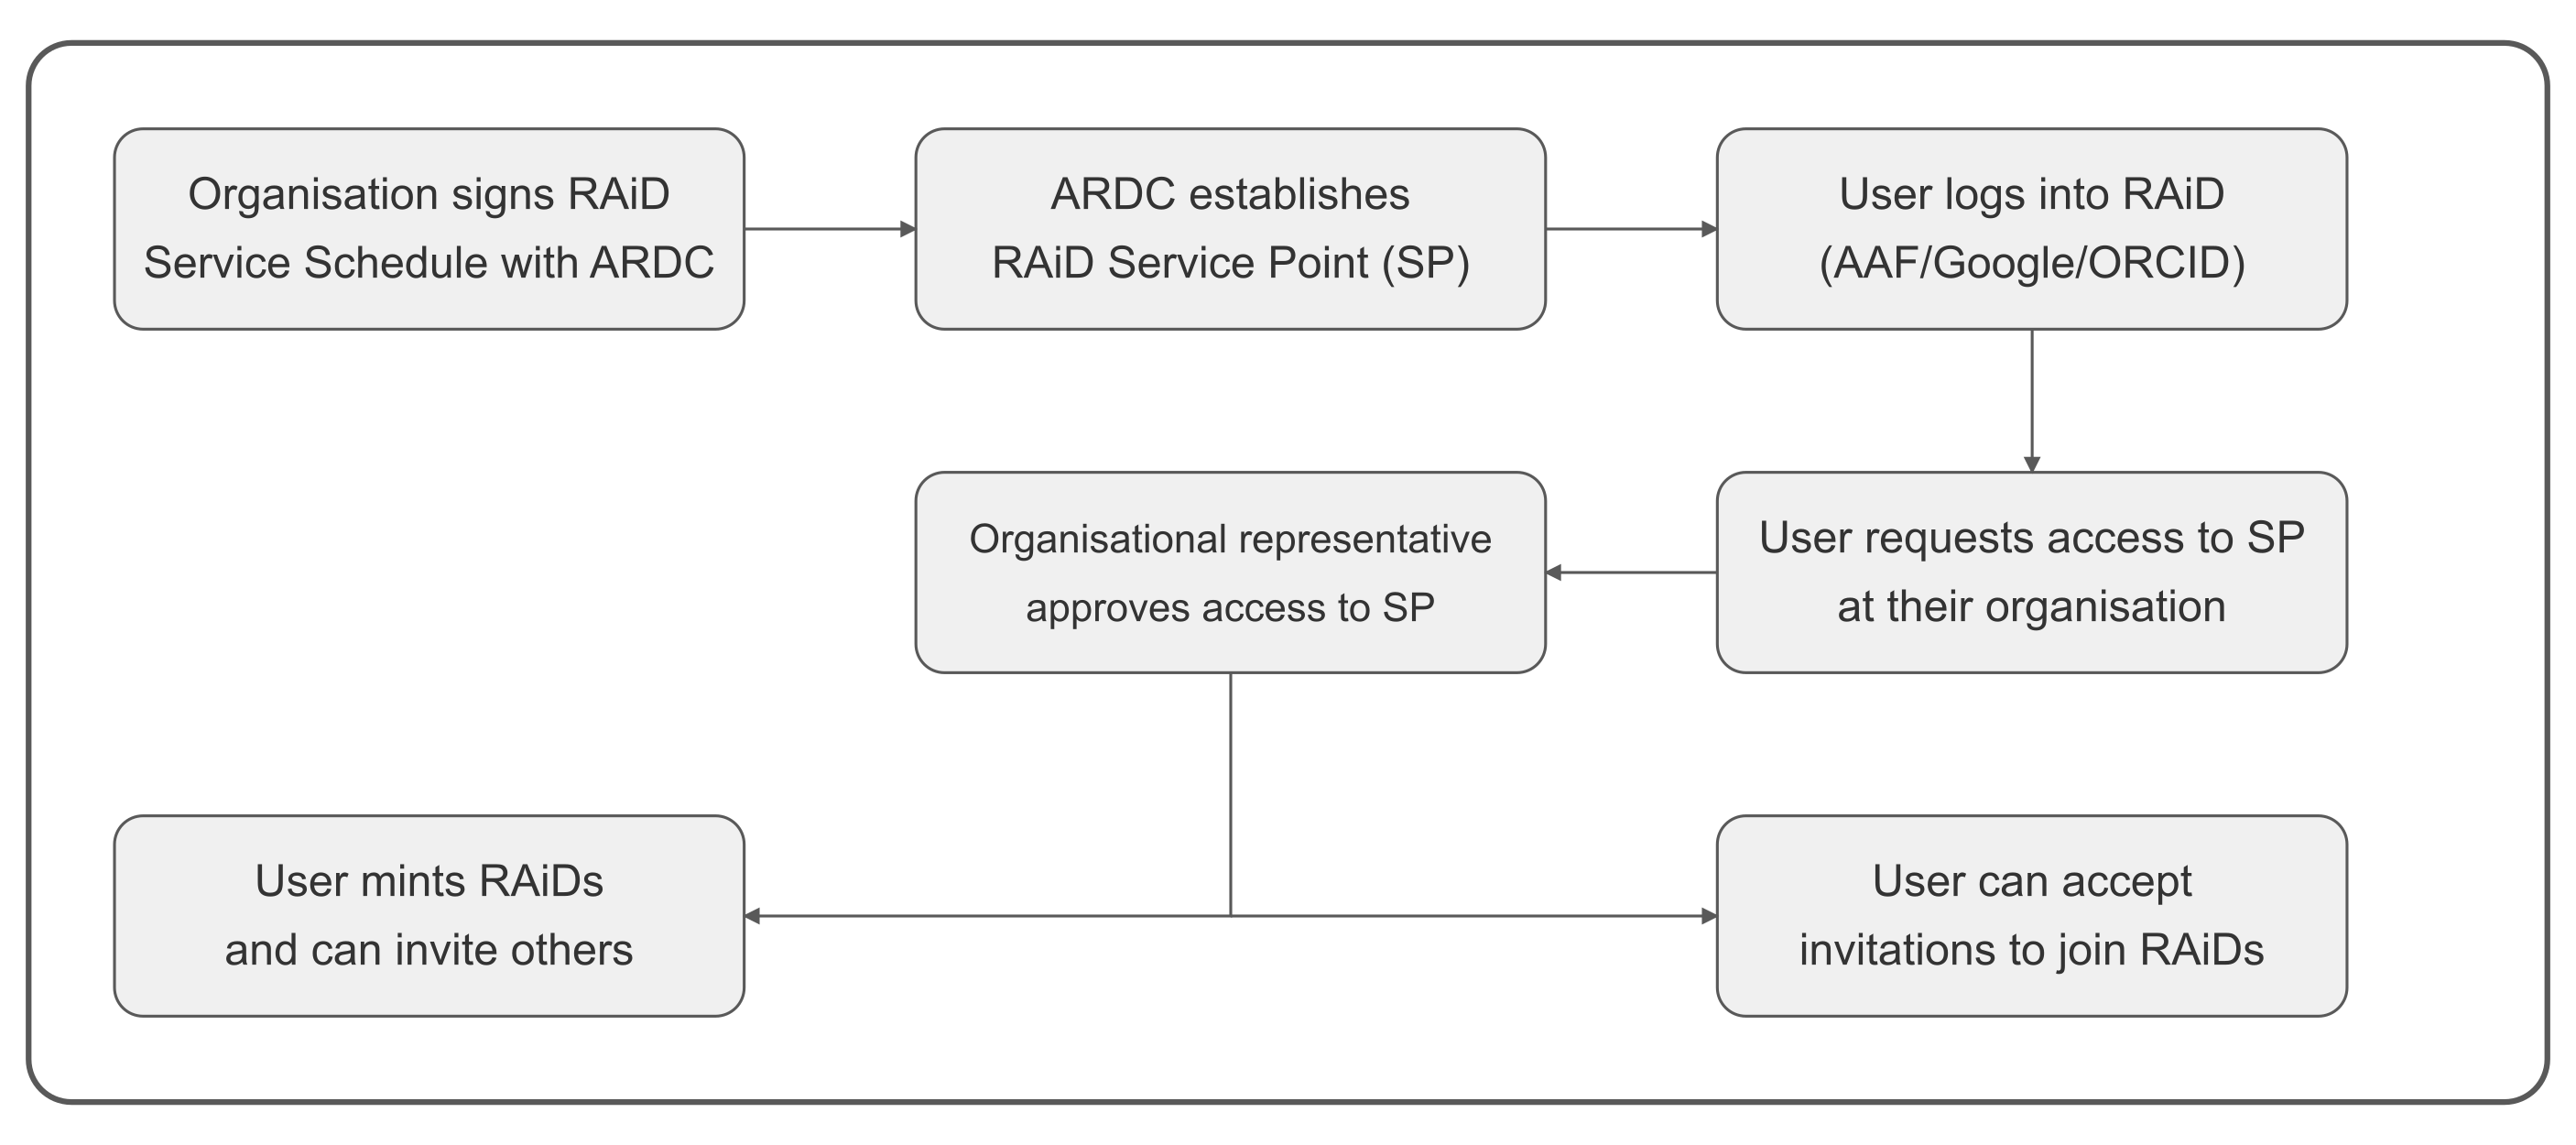
\includegraphics[width=0.9\linewidth]{figures/raid-workflow-anz.png}
 \captionof{figure}{Getting started with RAiD in Australia and New Zealand.}
 \label{raid-workflow}
\end{Figure}

%----------------------------------------------------------------------------------------
% 'Getting started with RAiD in Europe' figure  - STILL NEEDED
%----------------------------------------------------------------------------------------

\vspace{1cm}

\begin{wrapfigure}{r}{0.08\columnwidth}
    \vspace{-1.25cm}  % Adjust as needed for top spacing
    
\includegraphics[width=0.08\columnwidth]{figures/QR-code.png}
    \vspace{0.5cm}  % Adjust as needed for bottom spacing
\end{wrapfigure}
\hspace{1cm}  % Adjust as needed for horizontal spacing


\large{To try RAiD, please visit our \href{https://app.demo.raid.org.au/}{demo web app} (authenticate and then request access to the ‘RAiD Sandbox’ Service Point), or investigate our API \href{https://api.demo.raid.org.au/swagger-ui/index.html\#/}{https://api.demo.raid.org.au/swagger-ui/index.html\#/} (API token available via the web app).
}
%----------------------------------------------------------------------------------------
% RAID Metadata schema
%----------------------------------------------------------------------------------------

\vspace{-1cm}

\color{ARDCPink}
\section*{\LARGE RAiD metadata}
\color{DarkGrey}
\large{
\input schema
}

%----------------------------------------------------------------------------------------
% RAID Example
%----------------------------------------------------------------------------------------

\color{ARDCYellow}
\section*{\LARGE Example RAiD (excerpt)}
\color{DarkGrey}
\large{
Note that every controlled vocabulary declares a schema's URL (omitted here after a few examples) .
}

\small{
\input example
}

\end{multicols}

\vfill

%----------------------------------------------------------------------------------------
% LICENSE
%----------------------------------------------------------------------------------------

\begin{center}
\begin{tabular}{cc}
\raisebox{-0.2\height}{
\includegraphics[height=1cm]{cc-by.png}} &
\raisebox{0.2ex}{\small This work is licensed under a Creative Commons Attribution 4.0 International License.}
\end{tabular}
\end{center}

\end{document}